\section{Порядок выполнения лабораторной работы №3}
\begin{enumerate}
\item Выбрать вариант задания в приложении \ref{Lab3Var} в соответствии с номером в журнале.
\item Создать в папке с номером группы на рабочем столе папку \verb#Lab3# для файлов проекта.
\item Скопировать в созданную папку \verb#Lab3#, папку  \verb#CMSIS# из папки  \verb#LabWorkSTM32L/Materials# на рабочем столе.
\item Скопировать в созданную папку \verb#Lab3#, папку  \verb#STM32L1xx_StdPeriph_Driver# из папки  \verb#LabWorkSTM32L/Materials# на рабочем столе.
\item Скопировать в созданную папку \verb#Lab3#, папку  \verb#STM32_TouchSensing_Drive# из папки  \verb#LabWorkSTM32L/Materials# на рабочем столе.
\item Скопировать в созданную папку \verb#Lab3#, папку  \verb#Discovery# из папки  \verb#LabWorkSTM32L/Materials# на рабочем столе.
\item Скопировать в созданную папку \verb#Lab3# файлы \verb\stm32_tsl_conf.h\, \verb\stm32l1xx_conf.h\ из папки  \verb#LabWorkSTM32L/Materials# на рабочем столе.
\item Создать и настроить проект в среде разработки IAR.
\item В настройках проекта в категории \textit{C/C++ Compiler} во вкладке \textit{Preprocessor} указать путь до всех вложенных папок в папке \verb#Lab3#, заменяя Lab3 на \verb#$PROJ_DIR$# (см. лаб.1).
\item В качестве имени проекта указать \textit{lab3}, все файлы настроек проекта сохранить в папке \verb#Lab3#.
\item Добавить в проект все файлы библиотеки \textit{TSL} (папка \verb#STM32_TouchSensing_Driver#), все файлы из папки \verb#Discovery#.
\item Добавьте в проект файлы \verb\stm32_tsl_conf.h\, \verb\stm32l1xx_conf.h\.
\item Добавьте в проект файлы \verb\stm32l1xx_gpio.h\, \verb\stm32l1xx_rcc.h\, \verb\stm32l1xx_lcd.h\, \verb\stm32l1xx_exti.h\, \verb\stm32l1xx_gpio.c\, \verb\stm32l1xx_rcc.c\, \verb\stm32l1xx_lcd.c\, \verb\stm32l1xx_exti.c\ из \textit{SPL} (папка \verb#STM32L1xx_StdPeriph_Driver#).
\item В добавленные файлы из папки \verb#STM32L1xx_StdPeriph_Driver# добавить
\begin{verbatim}
#include "stm32l1xx_conf.h"
\end{verbatim}
\item Добавить в проект файлы \verb\system_stm32l1xx.h\, \verb\system_stm32l1xx.c\, \verb\stm32l1xx.h\ из папки \verb#LabWorkSTM32L/#
\verb#Materials/CMSIS/DeviceSupport/ST/STM32L1xx#.
\item Добавьте в проект файл \verb\startup_stm32l1xx_md.s\ из папки \verb#LabWorkSTM32L/Materials CMSIS/#
\verb#CM3/DeviceSupport/ST/STM32L1xx/startup/iar#
\item Добавить в проект файлы все файлы из папки \verb#Discovery#
\item Написать программу для микроконтроллера на языке Си.
\item Изменить функции \verb\Button_value()\ и \verb\Slider_value()\  в файле \verb\discover_functions.c\ в соответствии с вариантом задания.
\item Подключить отладочную плату STM32L - Discovery к компьютеру.
\item Загрузить программу в микроконтроллер и произвести ее отладку. 
\item Составить отчет.
\end{enumerate}

\section{Пример выполнения лабораторной работы №3}
Разработать программу в среде IAR. Режимы работы периферии приведены в таблице. В первом столбце приведены положения пользовательской кнопки \textit{USER} (количество соответствующих нажатий). Во втором столбце режимы работы сенсорной панели (слайдер или четыре раздельные кнопки). Третий столбец определена информация, выводимая на ЖКИ. Четвертый и пятый столбцы указывают режимы работы для светодиодов.

\begin{table}[h]
\caption{Задание к лабораторной работе}
\begin{tabular}{|c|c|c|c|c|}
\hline
\begin{tabular}[c]{@{}c@{}}Положение кнопки\\ User\end{tabular} & Сенсорная панель & ЖКИ   & Синий светодиод & Зеленый светодиод \\ \hline
\multirow{4}{*}{0}                                              & 0                & X000  &                 & Горит             \\ \cline{2-5} 
                                                                & 1                & 0X00  & Горит           &                   \\ \cline{2-5} 
                                                                & 2                & 00X0  & Горит           & Горит             \\ \cline{2-5} 
                                                                & 3                & 000X  &                 &                   \\ \hline
1                                                               & Слайдер          & X \%  &                 &                   \\ \hline
2                                                               &                  & GREEN &                 & Мигает            \\ \hline
3                                                               &                  & BLUE  & Мигает          &                   \\ \hline
\end{tabular}
\end{table}


\begin{figure}[H]
\begin{center}
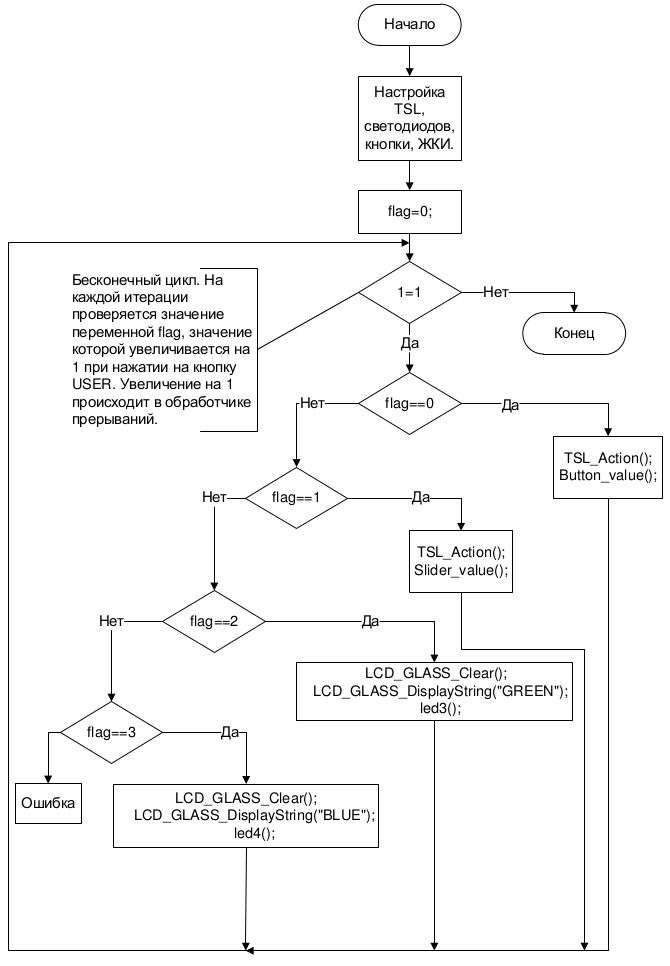
\includegraphics[scale=0.7]{Image/89.jpg} 
\end{center}
\caption{Блок схема алгоритма главной программы}
\end{figure}

\begin{figure}[H]
\begin{center}
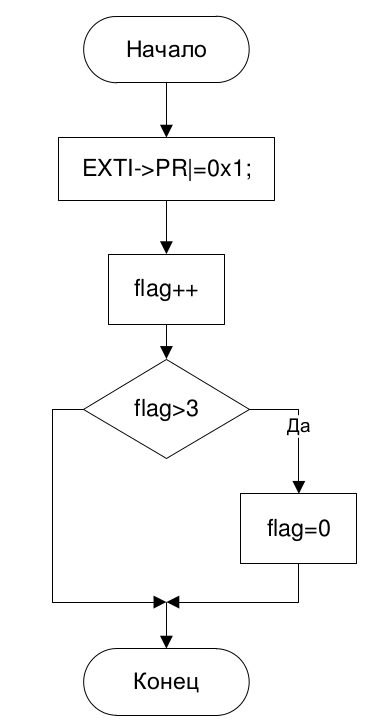
\includegraphics[scale=0.4]{Image/90.jpg} 
\end{center}
\caption{Блок схема алгоритма обработчика прерываний}
\end{figure}

\subsection{Пример главной программы для микроконтроллера}
\begin{verbatim}
/*################## Секция include ##################*/
#include "stm32l1xx_rcc.h"
#include "stm32l1xx_gpio.h"

#include "stm32_tsl_api.h"          /* API для работы с TSL */

#include "discover_functions.h"     /* Функции для работы с сенсорной 
                                       панелью */
#include "stm32l_discovery_lcd.h"   /* Функции для работы с ЖКИ */

/*################## Локальные переменные ##################*/
static uint32_t flag = 0;
static uint32_t TimingDelay;

/*################## Прототипы функций ##################*/
void LCD_GPIO_Init(void);
void LCD_CONTR_Init(void);
void LAB3_Delay(uint32_t);
void LED3_Blink(void);
void LED4_Blink(void);
void handler(void);
void LED_BUTTON_GPIO_Init(void);
void Interrupt_Init(void);
void TOUCH_PANEL_Init(void);

/*################## Опредение функций ##################*/

/*
 * Функция инициализации портов микроконтроллера, подключенных к LCD
 */
void LCD_GPIO_Init(void)
{
    /* Тактирование*/
    RCC->AHBENR |= (RCC_AHBENR_GPIOAEN | RCC_AHBENR_GPIOBEN | 
                    RCC_AHBENR_GPIOCEN);
    
    /* Режим работы, порты PA1 – PA3, PA8 – PA10, PA15 */
    GPIOA->MODER |= (GPIO_MODER_MODER1_1 | GPIO_MODER_MODER2_1 | 
                     GPIO_MODER_MODER3_1 | GPIO_MODER_MODER8_1 | 
                     GPIO_MODER_MODER9_1 | GPIO_MODER_MODER10_1 | 
                     GPIO_MODER_MODER15_1); 
    
    /* Режим работы, порты PB3 – PB5, PB8 – PB15 */
    GPIOB->MODER |= (GPIO_MODER_MODER3_1 | GPIO_MODER_MODER1_1 | 
                     GPIO_MODER_MODER5_1 | GPIO_MODER_MODER8_1 | 
                     GPIO_MODER_MODER9_1 | GPIO_MODER_MODER10_1 | 
                     GPIO_MODER_MODER11_1 | GPIO_MODER_MODER12_1 |
                     GPIO_MODER_MODER13_1 | GPIO_MODER_MODER14_1 | 
                     GPIO_MODER_MODER15_1); 
    
    /* Режим работы, порты PC0 – PC3, PC6 – PC11 */
    GPIOC->MODER |= (GPIO_MODER_MODER0_1 | GPIO_MODER_MODER1_1 | 
                     GPIO_MODER_MODER2_1 | GPIO_MODER_MODER3_1 |
                     GPIO_MODER_MODER6_1 | GPIO_MODER_MODER7_1 | 
                     GPIO_MODER_MODER8_1 | GPIO_MODER_MODER9_1 |  
                     GPIO_MODER_MODER10_1 | GPIO_MODER_MODER11_1); 
    
    /* Режим push – pull, порты PA1 – PA3, PA8 – PA10, PA15 */                 
    GPIOA->OTYPER &= ~(GPIO_OTYPER_OT_1 | GPIO_OTYPER_OT_2 |
                       GPIO_OTYPER_OT_3 | GPIO_OTYPER_OT_8 |
                       GPIO_OTYPER_OT_9 | GPIO_OTYPER_OT_10 |
                       GPIO_OTYPER_OT_15);
    
    /* Режим push – pull, порты PB3 – PB5, PB8 – PB15 */
    GPIOB->OTYPER &= ~(GPIO_OTYPER_OT_3 | GPIO_OTYPER_OT_4 | 
                       GPIO_OTYPER_OT_5 | GPIO_OTYPER_OT_8 | 
                       GPIO_OTYPER_OT_9 | GPIO_OTYPER_OT_10| 
                       GPIO_OTYPER_OT_11 | GPIO_OTYPER_OT_12 |
                       GPIO_OTYPER_OT_13 | GPIO_OTYPER_OT_14 | 
                       GPIO_OTYPER_OT_15);
    
    /* Режим push – pull, порты PC0 – PC3, PC6 – PC11 */
    GPIOC->OTYPER &= ~(GPIO_OTYPER_OT_0 | GPIO_OTYPER_OT_1 | 
                       GPIO_OTYPER_OT_2 | GPIO_OTYPER_OT_3 |
                       GPIO_OTYPER_OT_6 | GPIO_OTYPER_OT_7 | 
                       GPIO_OTYPER_OT_8 | GPIO_OTYPER_OT_9 |  
                       GPIO_OTYPER_OT_10 | GPIO_OTYPER_OT_11);
    
    /* Отключения подтягивающих резисторов, порты PA1 – PA3, 
       PA8 – PA10, PA15 */
    GPIOA->PUPDR &= ~(GPIO_PUPDR_PUPDR1 | GPIO_PUPDR_PUPDR2 |
                      GPIO_PUPDR_PUPDR3 | GPIO_PUPDR_PUPDR8 |
                      GPIO_PUPDR_PUPDR9 | GPIO_PUPDR_PUPDR10 |
                      GPIO_PUPDR_PUPDR15);

    /* Отключения подтягивающих резисторов, порты PB3 – PB5, PB8 – PB15 */
    GPIOB->PUPDR &= ~(GPIO_PUPDR_PUPDR3 | GPIO_PUPDR_PUPDR4 | 
                      GPIO_PUPDR_PUPDR5 | GPIO_PUPDR_PUPDR8 | 
                      GPIO_PUPDR_PUPDR9 | GPIO_PUPDR_PUPDR10| 
                      GPIO_PUPDR_PUPDR11 | GPIO_PUPDR_PUPDR12 |
                      GPIO_PUPDR_PUPDR13 | GPIO_PUPDR_PUPDR14 | 
                      GPIO_PUPDR_PUPDR15);

    /* Отключения подтягивающих резисторов, порты PC0 – PC3, PC6 – PC11 */
    GPIOC->PUPDR &= ~(GPIO_PUPDR_PUPDR0 | GPIO_PUPDR_PUPDR1 | 
                      GPIO_PUPDR_PUPDR2 | GPIO_PUPDR_PUPDR3 |
                      GPIO_PUPDR_PUPDR6 | GPIO_PUPDR_PUPDR7 | 
                      GPIO_PUPDR_PUPDR8 | GPIO_PUPDR_PUPDR9 |  
                      GPIO_PUPDR_PUPDR10 | GPIO_PUPDR_PUPDR11);
    
    /* Частота вывода информации, порты PA1 – PA3, PA8 – PA10, PA15 */
    GPIOA->OSPEEDR &= ~(GPIO_OSPEEDER_OSPEEDR1 | GPIO_OSPEEDER_OSPEEDR2 |
                        GPIO_OSPEEDER_OSPEEDR3 | GPIO_OSPEEDER_OSPEEDR8 |
                        GPIO_OSPEEDER_OSPEEDR9 | GPIO_OSPEEDER_OSPEEDR10 |
                        GPIO_OSPEEDER_OSPEEDR15);

    /* Частота вывода информации, порты PB3 – PB5, PB8 – PB15 */
    GPIOB->OSPEEDR &= ~(GPIO_OSPEEDER_OSPEEDR3 | GPIO_OSPEEDER_OSPEEDR4 | 
                        GPIO_OSPEEDER_OSPEEDR5 | GPIO_OSPEEDER_OSPEEDR8 | 
                        GPIO_OSPEEDER_OSPEEDR9 | GPIO_OSPEEDER_OSPEEDR10| 
                        GPIO_OSPEEDER_OSPEEDR11 | GPIO_OSPEEDER_OSPEEDR12 |
                        GPIO_OSPEEDER_OSPEEDR13 | GPIO_OSPEEDER_OSPEEDR14 | 
                        GPIO_OSPEEDER_OSPEEDR15);

    /* Частота вывода информации, порты PC0 – PC3, PC6 – PC11 */
    GPIOC->OSPEEDR &= ~(GPIO_OSPEEDER_OSPEEDR0 | GPIO_OSPEEDER_OSPEEDR1 | 
                        GPIO_OSPEEDER_OSPEEDR2 | GPIO_OSPEEDER_OSPEEDR3 |
                        GPIO_OSPEEDER_OSPEEDR6 | GPIO_OSPEEDER_OSPEEDR7 | 
                        GPIO_OSPEEDER_OSPEEDR8 | GPIO_OSPEEDER_OSPEEDR9 |  
                        GPIO_OSPEEDER_OSPEEDR10 | GPIO_OSPEEDER_OSPEEDR11);

    /* Установка альтернативной функции */
    GPIOA->AFR[0] |= 0xBBB0;
    GPIOA->AFR[1] |= 0xB0000BBB;

    GPIOB->AFR[0] |= 0xBBB000;
    GPIOB->AFR[1] |= 0xBBBBBBBB;

    GPIOC->AFR[0] |= 0xBB00BBBB;
    GPIOC->AFR[1] |= 0xBBBB;
}

 /*
 * Функция инициализации контроллера ЖКИ
 */
void LCD_CONTR_Init(void)
{
    /* Выбрать внутренний ВЧ генератор (HSI) */
    RCC->CR |= RCC_CR_HSION;

    /* Готовность HSI */
    while(!(RCC->CR&RCC_CR_HSIRDY));

    /* Выбор внутреннего ВЧ генератора в качестве источника 
       тактового сигнала */
    RCC->CFGR |= RCC_CFGR_SW_0;;

    /* Тактирование контроллера ЖКИ, системы управления питанием, 
       компаратора */
    RCC->APB1ENR |= (RCC_APB1ENR_PWREN | RCC_APB1ENR_LCDEN | 
                     RCC_APB1ENR_COMPEN);

    /* Снимается защита от записи в регистр RCC_CSR */
    PWR->CR |= PWR_CR_DBP;

    /* Сброс источника тактирования */
    RCC->CSR |= RCC_CSR_RTCRST;
    RCC->CSR &= ~RCC_CSR_RTCRST;

    /* Выбираем LSE (low-speed external) — 
       низкочастотный внешний источник */
    RCC->CSR |= RCC_CSR_LSEON;

    /* Ждем стабилизацию генератора */
    while(!(RCC->CSR&RCC_CSR_LSERDY));

    /* Выбор внешнего НЧ генератора в качестве источника 
       тактового сигнала */
    RCC->CSR |= RCC_CSR_RTCSEL_LSE;

    /* Установка bias = 1/3 */
    LCD->CR &= ~LCD_CR_BIAS;
    LCD->CR |= LCD_CR_BIAS_1;

    /* Установка duty = 1/3 */
    LCD->CR &= ~LCD_CR_DUTY;
    LCD->CR |= LCD_CR_DUTY_0 | LCD_CR_DUTY_1;

    /* Используем ф-цию переназначения выводов */
    LCD->CR |= LCD_CR_MUX_SEG;

    /* Устанавливаем коэффициенты деления частоты тактового сигнала */
    LCD->FCR &= ~LCD_FCR_PS;
    LCD->FCR &= ~LCD_FCR_DIV;

    /* ck_ps = LCDCLK / 16, ck_div = ck_ps / 17 */
    LCD->FCR |= 0x1040000;

    /* Установка контрасности */
    LCD->FCR &= ~LCD_FCR_CC;
    LCD->FCR |= LCD_FCR_CC_1;

    /* Ждем синхронизацию регистра LCD_FCR */
    while(!(LCD->SR&LCD_SR_FCRSR));

    /* Внутренний step-up converter для формирования V_lcd */
    LCD->CR &= ~LCD_CR_VSEL;

    /* Разрешение работы ЖКИ контроллера */
    LCD->CR |= LCD_CR_LCDEN;

    /* Ждем готовность step-up converter */
    while(!(LCD->SR&LCD_SR_RDY));

    /* Ждем готовность ЖКИ контроллера */
    while(!(LCD->SR&LCD_SR_ENS));
}

/*
 * Программная задержка
 * Входные данные:
 *  nTime - время задержки [мс]
 */
void LAB3_Delay(uint32_t nTime)
{
    TimingDelay = nTime;
    while(TimingDelay != 0);
}

/*
 * Мигание светодиода LED3
 */
void LED3_Blink(void)
{
    GPIO_SetBits(GPIOB, GPIO_Pin_7);
    LAB3_Delay(250);

    GPIO_ResetBits(GPIOB, GPIO_Pin_7);
    LAB3_Delay(250);
}

/*
 * Мигание светодиода LED4
 */
void LED4_Blink(void)
{
    GPIO_SetBits(GPIOB, GPIO_Pin_6);
    LAB3_Delay(250);

    GPIO_ResetBits(GPIOB, GPIO_Pin_6);
    LAB3_Delay(250);
}

/*
 *  Обработчик прерывания нажатия на кнопку
 */
void EXTI0_IRQHandler(void)
{
    EXTI->PR |= 0x01; /* Сброс бита события, вызвавшего прерывание */
    flag++;
    if (flag > 3)
    {
        flag = 0;
    }
}


/*
 * Обработчик прерывания системного таймера
 * Вызов функции SysTick_Config() определенной в core_cm3.h
 * происходит в файле stm32_tsl_timebase.c
 */

void SysTick_Handler(void)
{
    if (TimingDelay != 0x00)
    {
        TimingDelay--;
    }
}

/*
 * Настройка светодиодов и кнопки USER
 */
void LED_BUTTON_GPIO_Init(void)
{
    GPIO_InitTypeDef GPIO_InitStructure;
    
    RCC_AHBPeriphClockCmd(RCC_AHBPeriph_GPIOB, ENABLE);

    /* Настройка светодиодов */
    GPIO_InitStructure.GPIO_Pin = GPIO_Pin_7 | GPIO_Pin_6 ;
    GPIO_InitStructure.GPIO_Mode = GPIO_Mode_OUT;
    GPIO_InitStructure.GPIO_Speed = GPIO_Speed_400KHz;
    GPIO_InitStructure.GPIO_OType = GPIO_OType_PP;
    
    GPIO_Init(GPIOB, &GPIO_InitStructure);

    /* Настройка кнопки USER */
    GPIO_InitStructure.GPIO_Pin = GPIO_Pin_0;
    GPIO_InitStructure.GPIO_Mode = GPIO_Mode_IN;
    GPIO_InitStructure.GPIO_PuPd = GPIO_PuPd_NOPULL;
    GPIO_InitStructure.GPIO_Speed = GPIO_Speed_40MHz;
    
    GPIO_Init(GPIOA, &GPIO_InitStructure);
}

/*
 * Настройка прерываний
 */
void Interrupt_Init(void)
{
    EXTI->IMR |= EXTI_IMR_MR0;
    EXTI->RTSR |= EXTI_RTSR_TR0;
    NVIC_EnableIRQ (EXTI0_IRQn);
}
  
/*
 * Настройка сенсорной панели
 */  
void TOUCH_PANEL_Init(void)
{
    TSL_Init();
    sMCKeyInfo[0].Setting.b.IMPLEMENTED = 1;
    sMCKeyInfo[0].Setting.b.ENABLED = 1;
    sMCKeyInfo[0].DxSGroup = 0x00;
}

/*################## Программа ##################*/
void main(void)
{
    Interrupt_Init()

    TOUCH_PANEL_Init();

    LED_BUTTON_GPIO_Init();

    LCD_GPIO_Init();
    LCD_CONTR_Init();

    while(1)
    {
        switch (flag)
        {
            case 0:
                TSL_Action();

                /* Сенсорная панель как 4 раздельные кнопки */
                Button_value(); 
                break;
            case 1:
                TSL_Action();

                /* Сенсорная панель как слайдер */
                Slider_value(); 
                break;
            case 2:
                LCD_GLASS_Clear();
                LCD_GLASS_DisplayString("GREEN");
                LED3_Blink();
                break;
            case 3:
                LCD_GLASS_Clear();
                LCD_GLASS_DisplayString("BLUE");
                LED4_Blink();
                break; 
        }
    } /* end of while(1) */
} /* end of main() */
\end{verbatim}

\subsection{Пример изменения файла discover\_functions.c}
STMicroelectronics поставляет вместе с отладочной платой набор функций по работе с сенсорной панелью. Чтобы не переписывать заново функции работы с сенсорной панелью, в данной лабораторной работе нужно изменить функции \verb\Slider_value()\ и \verb\Button_value()\ в соответствии с вариантом задания
\begin{verbatim}
/*
 * Вывод точки касания в процентах
 */ 
void Slider_value(void)
{
    uint16_t Message[6];  
    uint32_t percent_value;

    GPIO_ResetBits(GPIOB, GPIO_Pin_6);
    GPIO_ResetBits(GPIOB, GPIO_Pin_7);
   
    /*В массив Massage[] заносятся символы для отображения на ЖКИ */ 
    Message[0] = ' ';
    Message[1] = ' ';
    Message[2] = ' ';

    if ((TSL_GlobalSetting.b.CHANGED) && (TSLState == TSL_IDLE_STATE)) 
    {
        TSL_GlobalSetting.b.CHANGED = 0;
    }
    
    if ((SLIDER_DETECTED) && (TSLState == TSL_IDLE_STATE))
    {   
        /* Если касание обнаружено */ 
        percent_value = SLIDER_POSITION ;
        percent_value *= 10000;
        percent_value /= 255 ;    

        convert_into_char(percent_value,Message);

        Message[3] = '0' ;
        Message[4] = '/' ;
        Message[5] = '%' ;

        /* Вывод на ЖКИ в виде "X %", где Х - положение точки касания */
        LCD_GLASS_DisplayStrDeci(Message);
    } 
    else if((!TSL_GlobalSetting.b.CHANGED) && (TSLState == TSL_IDLE_STATE))
    {     
          /* Если касание не обнаружено */
          Message[3] = '0' ;
          Message[4] = '/' ;
          Message[5] = '%' ;   
          LCD_GLASS_DisplayStrDeci(Message);
    } 
}

/*
 * Сенсорная панель как 4 раздельные кнопки
 */
void Button_value(void)
{
    uint8_t Message[6];  

    /*В массив Massage[] заносятся символы для отображения на ЖКИ */   
    Message[0] = ' ';
    Message[1] = '0';
    Message[2] = '0';
    Message[3] = '0';
    Message[4] = '0';
    Message[5] = ' ';
      
    if ((TSL_GlobalSetting.b.CHANGED) && (TSLState == TSL_IDLE_STATE)) 
    {
        TSL_GlobalSetting.b.CHANGED = 0;
    }

    if ((SLIDER_DETECTED) && (TSLState == TSL_IDLE_STATE))
    {
        /* Если касание обнаружено */
        /* Вся область сенсорной панели делится на 4 части 
           определением точки касания */  
        if( SLIDER_POSITION <= 25 )
        {
          Message[1] = 255;       
          GPIO_SetBits(GPIOB, GPIO_Pin_7);
          GPIO_ResetBits(GPIOB, GPIO_Pin_6);
        }
        
        if( (SLIDER_POSITION > 25 ) && (SLIDER_POSITION <= 110 )) 
        {       
          Message[2] = 255; 
          GPIO_ResetBits(GPIOB, GPIO_Pin_7);
          GPIO_SetBits(GPIOB, GPIO_Pin_6);  
        }
        
        if( (SLIDER_POSITION > 110 ) && (SLIDER_POSITION <= 200 )) 
        {      
          Message[3] = 255;  
          GPIO_SetBits(GPIOB, GPIO_Pin_6);
          GPIO_SetBits(GPIOB, GPIO_Pin_7); 
        }
        
        if( SLIDER_POSITION > 200 )
        {    
          Message[4] = 255;
          GPIO_ResetBits(GPIOB, GPIO_Pin_6);
          GPIO_ResetBits(GPIOB, GPIO_Pin_7);

        }
          
        /*Вывод на ЖКИ в виде "0Х00", где Х - положение точки касания */   
        LCD_GLASS_DisplayString(Message);
    } 
    else if((!TSL_GlobalSetting.b.CHANGED) && (TSLState == TSL_IDLE_STATE))
    {     
        /* Если касание не обнаружено */
        LCD_GLASS_DisplayString(Message);
    }
}
\end{verbatim}


\section{Варианты заданий к лабораторной работе №3}

\begin{table}[h]
\caption{Вариант 1}
\begin{tabular}{|c|c|c|c|c|}
\hline
\begin{tabular}[c]{@{}c@{}}Положение кнопки\\ User\end{tabular} & Сенсорная панель & ЖКИ   & Синий светодиод & Зеленый светодиод \\ \hline
0                                                               &                  &       & Мигает          & Мигает            \\ \hline
\multirow{4}{*}{1}                                              & 0                & VAR 1 &                 &                   \\ \cline{2-5} 
                                                                & 1                &       & Горит           &                   \\ \cline{2-5} 
                                                                & 2                &       &                 &                   \\ \cline{2-5} 
                                                                & 3                &       &                 & Горит             \\ \hline
2                                                               &                  &       & Горит           &                   \\ \hline
3                                                               & Слайдер          & X \%  &                 &                   \\ \hline
\end{tabular}
\end{table}

\begin{table}[h]
\caption{Вариант 2}
\begin{tabular}{|c|c|c|c|c|}
\hline
\begin{tabular}[c]{@{}c@{}}Положение кнопки\\ User\end{tabular} & Сенсорная панель & ЖКИ   & Синий светодиод & Зеленый светодиод \\ \hline
0                                                               & Слайдер          & X \%  & Горит           &                   \\ \hline
1                                                               &                  &       &                 &                   \\ \hline
\multirow{4}{*}{2}                                              & 0                &       & Горит           & Мигает            \\ \cline{2-5} 
                                                                & 1                & VAR 2 &                 &                   \\ \cline{2-5} 
                                                                & 2                &       &                 & Мигает            \\ \cline{2-5} 
                                                                & 3                &       & Горит           &                   \\ \hline
3                                                               &                  &       &                 &                   \\ \hline
\end{tabular}
\end{table}

\begin{table}[h]
\caption{Вариант 3}
\begin{tabular}{|c|c|c|c|c|}
\hline
\begin{tabular}[c]{@{}c@{}}Положение кнопки\\ User\end{tabular} & Сенсорная панель & ЖКИ   & Синий светодиод & Зеленый светодиод \\ \hline
0                                                               & Слайдер          & X \%  &                 &                   \\ \hline
1                                                               &                  & VAR 3 & Горит           & Горит             \\ \hline
\multirow{4}{*}{2}                                              & 0                & KEY 1 &                 &                   \\ \cline{2-5} 
                                                                & 1                & KEY 2 &                 &                   \\ \cline{2-5} 
                                                                & 2                & KEY 3 &                 &                   \\ \cline{2-5} 
                                                                & 3                & KEY 1 &                 &                   \\ \hline
3                                                               &                  &       & Мигает          & Горит             \\ \hline
\end{tabular}
\end{table}

\begin{table}[h]
\caption{Вариант 4}
\begin{tabular}{|c|c|c|c|c|}
\hline
\begin{tabular}[c]{@{}c@{}}Положение кнопки\\ User\end{tabular} & Сенсорная панель & ЖКИ  & Синий светодиод & Зеленый светодиод \\ \hline
0                                                               &                  & ALL  & Горит           & Горит             \\ \hline
1                                                               &                  & NULL &                 &                   \\ \hline
\multirow{4}{*}{2}                                              & 0                &      &                 & Горит             \\ \cline{2-5} 
                                                                & 1                &      & Мигает          &                   \\ \cline{2-5} 
                                                                & 2                &      &                 & Горит             \\ \cline{2-5} 
                                                                &                  &      & Мигает          &                   \\ \hline
3                                                               & Слайдер          & X \% &                 &                   \\ \hline
\end{tabular}
\end{table}


\begin{table}[h]
\caption{Вариант 5}
\begin{tabular}{|c|c|c|c|c|}
\hline
\begin{tabular}[c]{@{}c@{}}Положение кнопки\\ User\end{tabular} & Сенсорная панель & ЖКИ  & Синий светодиод & Зеленый светодиод \\ \hline
0                                                               &                  &      &                 & Горит             \\ \hline
1                                                               & Слайдер          & X \% &                 &                   \\ \hline
2                                                               &                  &      & Мигает          &                   \\ \hline
\multirow{4}{*}{3}                                              & 0                & ALL  & Мигает          & Мигает            \\ \cline{2-5} 
                                                                & 1                &      & Горит           &                   \\ \cline{2-5} 
                                                                & 2                &      &                 & Горит             \\ \cline{2-5} 
                                                                & 3                &      & Мигает          &                   \\ \hline
\end{tabular}
\end{table}


\begin{table}[h]
\caption{Вариант 6}
\begin{tabular}{|c|c|c|c|c|}
\hline
\begin{tabular}[c]{@{}c@{}}Положение кнопки\\ User\end{tabular} & Сенсорная панель & ЖКИ  & Синий светодиод & Зеленый светодиод \\ \hline
0                                                               & Слайдер          & X \% &                 & Горит             \\ \hline
1                                                               &                  &      &                 &                   \\ \hline
2                                                               &                  &      &                 & Горит             \\ \hline
\multirow{4}{*}{3}                                              & 0                &      & Мигает          & Мигает            \\ \cline{2-5} 
                                                                & 1                &      &                 &                   \\ \cline{2-5} 
                                                                & 2                & ALL  & Горит           & Горит             \\ \cline{2-5} 
                                                                & 3                &      & Мигает          &                   \\ \hline
\end{tabular}
\end{table}

\begin{table}[h]
\caption{Вариант 7}
\begin{tabular}{|c|c|c|c|c|}
\hline
\begin{tabular}[c]{@{}c@{}}Положение кнопки\\ User\end{tabular} & Сенсорная панель & ЖКИ   & Синий светодиод & Зеленый светодиод \\ \hline
\multirow{4}{*}{0}                                              & 0                & GREEN &                 & Горит             \\ \cline{2-5} 
                                                                & 1                &       &                 &                   \\ \cline{2-5} 
                                                                & 2                &       & Горит           &                   \\ \cline{2-5} 
                                                                & 3                &       & Мигает          &                   \\ \hline
1                                                               &                  &       &                 &                   \\ \hline
2                                                               & Слайдер          & X \%  &                 & Горит             \\ \hline
3                                                               &                  &       &                 & Горит             \\ \hline
\end{tabular}
\end{table}

\begin{table}[h]
\caption{Вариант 8}
\begin{tabular}{|c|c|c|c|c|}
\hline
\begin{tabular}[c]{@{}c@{}}Положение кнопки\\ User\end{tabular} & Сенсорная панель & ЖКИ   & Синий светодиод & Зеленый светодиод \\ \hline
\multirow{4}{*}{0}                                              & 0                &       &                 & Мигает            \\ \cline{2-5} 
                                                                & 1                & NULL  &                 &                   \\ \cline{2-5} 
                                                                & 2                & ALL   & Мигает          & Мигает            \\ \cline{2-5} 
                                                                & 3                & GREEN &                 & Горит             \\ \hline
1                                                               & Слайдер          & X \%  &                 &                   \\ \hline
2                                                               &                  &       & Мигает          &                   \\ \hline
3                                                               &                  &       & Мигает          &                   \\ \hline
\end{tabular}
\end{table}

\begin{table}[h]
\caption{Вариант 9}
\begin{tabular}{|c|c|c|c|c|}
\hline
\begin{tabular}[c]{@{}c@{}}Положение кнопки\\ User\end{tabular} & Сенсорная панель & ЖКИ  & Синий светодиод & Зеленый светодиод \\ \hline
0                                                               &                  &      & Мигает          &                   \\ \hline
\multirow{4}{*}{1}                                              & 0                &      &                 & Горит             \\ \cline{2-5} 
                                                                & 1                &      &                 &                   \\ \cline{2-5} 
                                                                & 2                &      & Горит           &                   \\ \cline{2-5} 
                                                                & 3                &      &                 & Горит             \\ \hline
2                                                               &                  & ALL  & Мигает          & Мигает            \\ \hline
3                                                               & Слайдер          & X \% & Мигает          &                   \\ \hline
\end{tabular}
\end{table}


\begin{table}[h]
\caption{Вариант 10}
\begin{tabular}{|c|c|c|c|c|}
\hline
\begin{tabular}[c]{@{}c@{}}Положение кнопки\\ User\end{tabular} & Сенсорная панель & ЖКИ   & Синий светодиод & Зеленый светодиод \\ \hline
0                                                               &                  &       & Горит           & Горит             \\ \hline
\multirow{4}{*}{1}                                              & 0                & KEY 1 &                 &                   \\ \cline{2-5} 
                                                                & 1                &       &                 &                   \\ \cline{2-5} 
                                                                & 2                &       & Мигает          & Мигает            \\ \cline{2-5} 
                                                                & 3                & BLUE  &                 &                   \\ \hline
2                                                               &                  & ALL   & Горит           &                   \\ \hline
3                                                               & Слайдер          & X \%  & Мигает          & Мигает            \\ \hline
\end{tabular}
\end{table}